\documentclass[11pt]{article}
\usepackage{amsmath}
\usepackage{graphicx}
\usepackage{multirow}
\usepackage{booktabs}
\usepackage{verbatim}
\usepackage{color}
\usepackage{hyperref}
\usepackage{url}
\usepackage{geometry}
\usepackage{esvect}
\usepackage{esdiff}
\usepackage{siunitx}
\usepackage{caption}
\usepackage{subfig}
\usepackage{textcomp, gensymb}
%\textwidth 17cm
%\evensidemargin -0.5cm
%\oddsidemargin -0.5cm
\geometry{margin=2.5cm}
\setlength{\belowcaptionskip}{-10pt}

%TITLE PAGE WITH ABSTRACT AND ToC
\begin{document}
\title{Ganymede Surface Magnetic Field Analysis}
\author{Isaac Wetton}
\date{\today}
\maketitle

\section{Introduction}
\label{sec:intro}

This document details how I went about analysing the surface magnetic field strength of Ganymede using observed magnetic field data from the Galileo spacecraft. Section \ref{sec:meth} will describe the method employed to obtain magnetic field data plots and a result for the magnetic field at the surface of Ganymede so that the results may be reproduced, whilst section \ref{sec:result} will analyse the obtained data to draw conclusions on the surface magnetic field strength, discuss uncertainty in the result and any additional factors.

\section{Methodology}
\label{sec:meth}

Galileo spacecraft data was chosen as Galileo was a Jupiter orbiter which recorded measurements of magnetic field strengths and made multiple flybys of Ganymede \cite{craft}. The magnetic field data recorded by Galileo, alongside data for its position with respect to Jupiter and Ganymede, were retrieved from the \emph{Amda} website \cite{amda}. To determine the surface magnetic field strength of Ganymede, we opted to use observed data from Galileo's flyby of the satellite on 27\textsuperscript{th} December 2000 \cite{nasaflybys} as it had more frequent and more consistent measurements in comparison to previous flybys, and flew near to Ganymede's southern pole.

The measurements taken of magnetic field during the flyby have contributions from both Jupiter and Ganymede. To isolate Ganymede's magnetic field from Jupiter's contribution, multiple Python scripts, available in appendix \ref{app:scripts}, were written to first identify time frames in which Galileo was in approximately the same position as it was during the December 2000 flyby, then to modify one of these occasions' data to produce artificial Jupiter field data which could be subtracted to isolate Ganymede's field during the flyby.

\subsection{Identifying occasions with a similar Galileo position to December 2000's flyby}
The first Python script used an input text file containing position data from \emph{Amda} for Galileo's orbit of Jupiter from 1\textsuperscript{st} September 1996 to 1\textsuperscript{st} September 2003. If the position of the spacecraft was within approximately 5 Jupiter radii in each JSO direction of its position during the December 2000 flyby of Ganymede, then that data point was added to an output file. The position of Galileo during the December 2000 flyby was taken as its average across the stated time frame \cite{nasaflybys}, measured to be (-15.2, 0.57, 0.84) in JSO coordinates \cite{amda}.

The script identified a total of 7 additional occasions where Galileo was within the specified position range: 9\textsuperscript{th} October 1999, 24\textsuperscript{th} November 1999, 2\textsuperscript{nd} January 2000, 21\textsuperscript{st} February 2000, 20\textsuperscript{th} May 2000, 22\textsuperscript{nd} May 2001 and 5\textsuperscript{th} August 2001, each having a duration of between 6.5 and 17.5 hours. Timeseries of observed magnetic field strength at Galileo for the first six of these occasions are shown in figure \ref{fig:6panelmag}.

\begin{figure}[!htb]
    \centering
    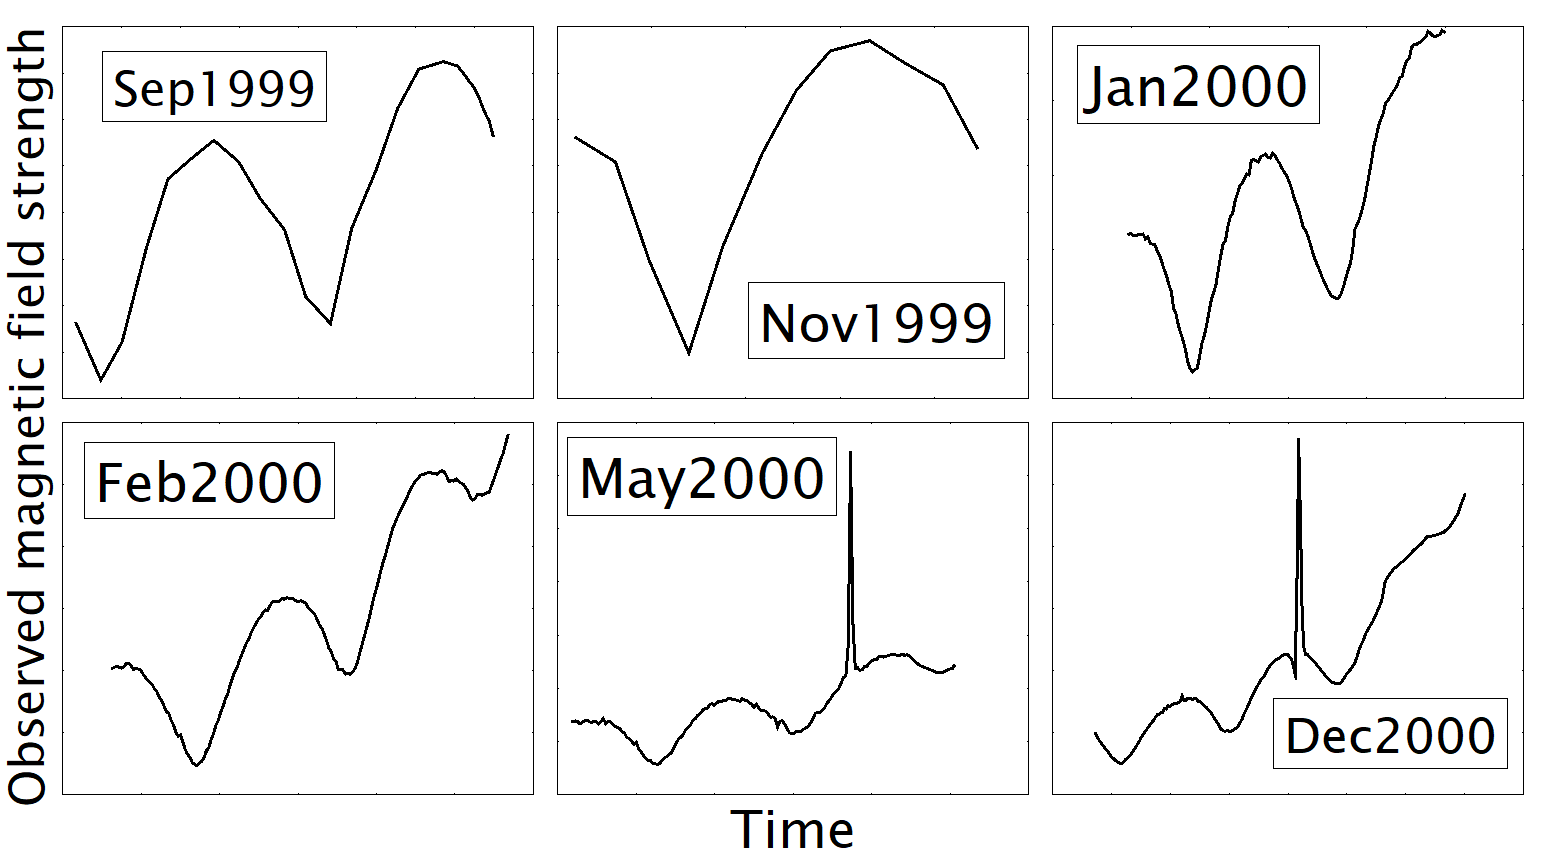
\includegraphics[width=8cm]{6magtimeseries-small.png}
    \captionsetup{width=13cm}
    \caption{Six timeseries of observed magnetic field magnitude by Galileo during six occasions where Galileo's position was similar to that of its December 2000 flyby of Ganymede. Moving across from top-left: 9\textsuperscript{th} October 1999, 24\textsuperscript{th} November 1999, 2\textsuperscript{nd} January 2000, 21\textsuperscript{st} February 2000, 20\textsuperscript{th} May 2000, 27\textsuperscript{th} December 2000.}
    \label{fig:6panelmag}
\end{figure}

\subsection{Isolating Ganymede's magnetic field from December 2000's flyby data}

Two new Python scripts were then written to remove Jupiter's contribution from the data. The May 2000 data was determined to have a non-flyby peak of similar magnitude to the December 2000 plot if the flyby spike was ignored, and so the script used May data to construct artificial December 2000 data for Jupiter's contribution only, which could then be subtracted from the December 2000 timeseries in figure \ref{fig:6panelmag} to effectively `isolate' Ganymede's field. The artificial data was created by calculating the difference between the May and December peaks when there was not a flyby, and adjusting the May data by the average distance. The script outputted an ASCII data file with values for time, magnetic field contribution and Galileo-Ganymede distance for the isolated Ganymede data.

Two plots were then produced - a timeseries of Ganymede's magnetic field contribution and a plot of Ganymede's magnetic field contribution against Galileo-Ganymede distance - for analysis of the field. The distance plot was solely for the Ganymede encounter period where there was a noticeable contribution from Ganymede, and included both the approach and retreat, with a fit of the form $\frac{A}{x^{3}} + B$ applied where $x$ is Galileo-Ganymede distance and $A$ and $B$ are constants. This particular fit was chosen as magnetic field strength from a dipole has an inverse cube law relationship with distance \cite{inversecube}, whilst also allowing for a potential base field due to other sources. The fit allowed for extrapolation to estimate the surface field at a distance of 1 Ganymede radius using the determined values of $A$ and $B$.

\subsection{Consideration of Ganymede's magnetic field rotation when comparing to expected results}

During the December 2000 flyby of Ganymede, Galileo flies close to the geographic north pole of Ganymede \cite{flybylines}. However, the magnetic north pole is rotated by $176 \pm 1\degree$ with respect to Jupiter's spin axis and $24 \pm 1\degree$ from the Jupiter-facing meridian plane toward the trailing hemisphere \cite{magrotation}. This must be accounted for to adjust the expected value before it can be compared to the surface field estimate we have obtained.

\subsection{Analysis of the May 2000 flyby data and estimation of surface magnetic field strength at Ganymede}
It can be seen from figure \ref{fig:6panelmag} that the May 2000 data also includes a flyby of Ganymede, characterised by the large spike in observed magnetic field strength at Galileo. This flyby specifically occurred on 2000-05-20 \cite{nasaflybys}, and occurred in a similar position with respect to Jupiter (within 5 Jupiter radii in each JSO coordinate as discussed) as the December 2000 flyby. The May flyby, however, crossed near to the geographic equator \cite{flybylines}.

The method used for obtaining a surface magnetic field strength at Ganymede for the December flyby was used to also obtain a value for the May flyby. The February 2000 data from approximately the same position with respect to Jupiter was used to create the artificial May data as it was determined to have a non-flyby peak of similar magnitude to the Jupiter field in May. The rotation of Ganymede's magnetic field was then taken into account and it was compared to the expected value from literature.

\section{Results \& Analysis}
\label{sec:result}

Reviewing the timeseries in \ref{fig:6panelmag}, it became apparent that the May 2000 and December 2000 plots were at far greater resolution to the other plots, particularly in comparison to the 1999 plots. It was known that the December 2000 Ganymede flyby, however it was found that the occasion where Galileo was in a similar position in May 2000 also included flyby-like magnetic field data, and was in fact during the time of a Ganymede flyby \cite{nasaflybys}. There were now two separate flyby dates which were observed from approximately the same position. Conveniently, the December flyby flew close to the geographic North pole of Ganymede whilst the May flyby flew nearby the geographic equator, as seen in figure \ref{fig:flybytrajectory}, allowing for the observation of both equatorial and polar magnetic field strength behaviour from similar positions.

\begin{figure}[!htb]
    \centering
    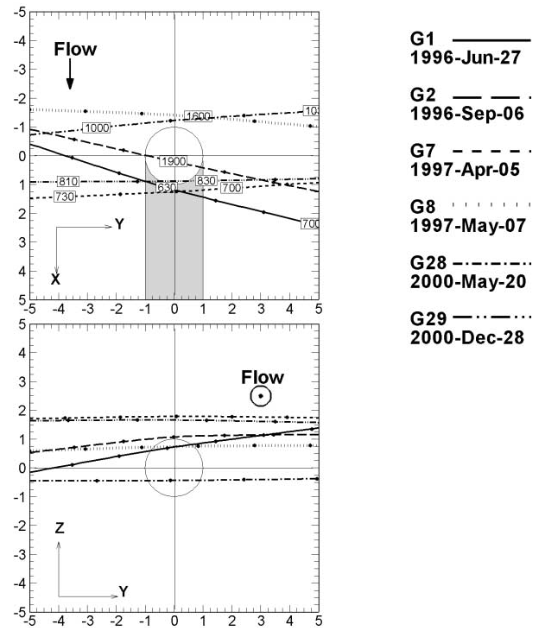
\includegraphics[width=6cm]{galtraj.png}
    \captionsetup{width=13cm}
    \caption{Plots of Galileo position with respect to Ganymede in GPhiO coordinates for six Ganymede flybys, including those in May and December 2000 \cite{magrotation}. X is in the direction of Ganymede's motion, Y is in the Ganymede-Jupiter axis, and Z is Ganymede's spin axis. The above plot shows X-Y position whilst the lower plot shows Z-Y position.}
    \label{fig:flybytrajectory}
\end{figure}

\newpage
\subsection{Removal of Jupiter's magnetic field contribution}

Data from February 2000 and May 2000 were used to construct artificial Jupiter contribution data for the flybys in May 2000 and December 2000 respectively. The removal of this contribution from the timeseries in figure \ref{fig:6panelmag} produced the plots of Ganymede's isolated magnetic field contribution shown in figures \ref{fig:isoMay} and \ref{fig:isoDec} for May 2000 and December 2000 respectively.

\begin{figure}[!htb]
    \centering
    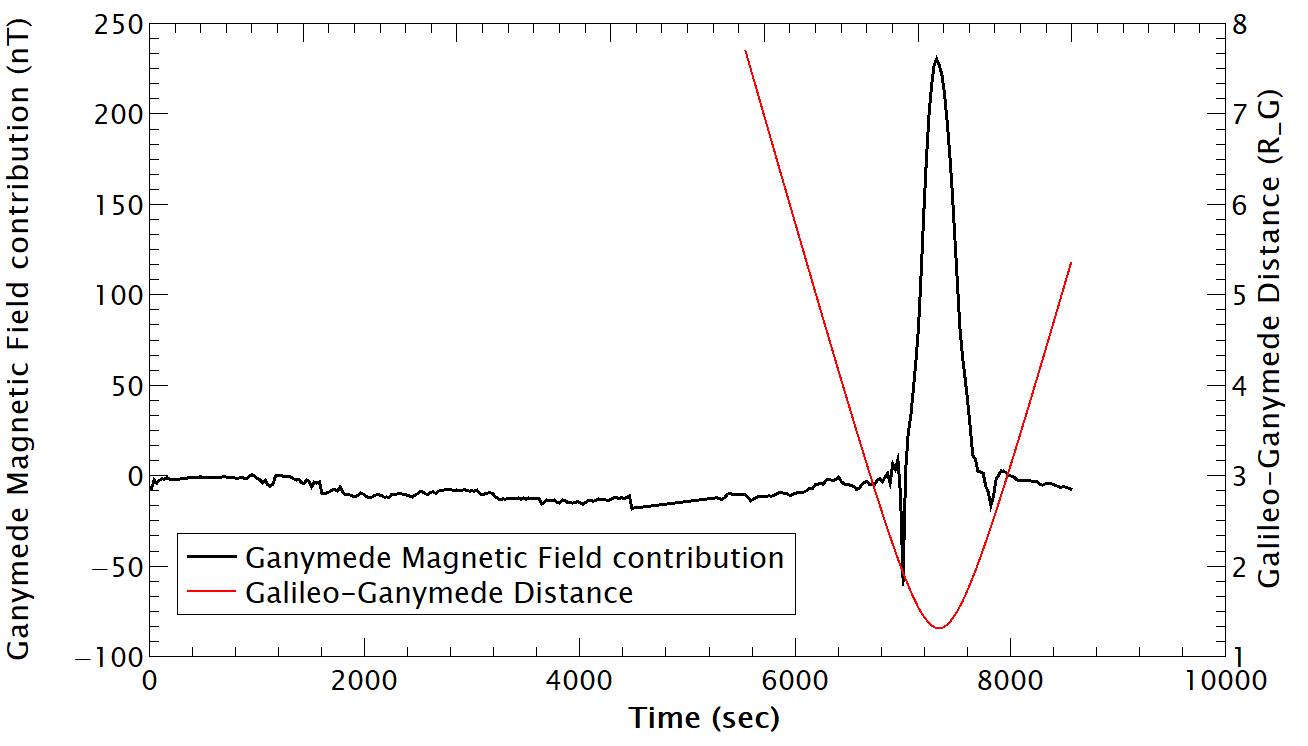
\includegraphics[width=8cm]{isoMay.png}
    \captionsetup{width=13cm}
    \caption{A timeseries of Ganymede's isolated magnetic field (measured in nT) observed by Galileo during its May 2000 flyby of the satellite, with artificial Jupiter magnetic field data removed from the overall magnetometer reading at Galileo, alongside available data for Galileo-Ganymede distance (measured in Ganymede radii).}
    \label{fig:isoMay}
\end{figure}

\begin{figure}[!htb]
    \centering
    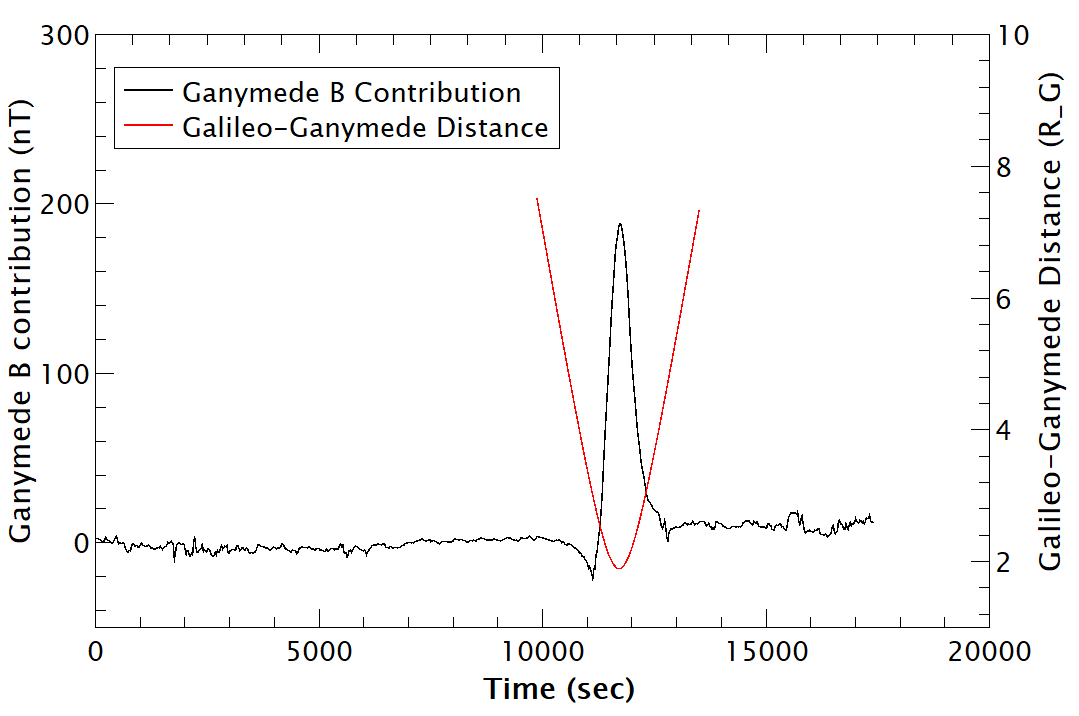
\includegraphics[width=8cm]{isoDec.png}
    \captionsetup{width=13cm}
    \caption{A timeseries of Ganymede's isolated magnetic field (measured in nT) observed by Galileo during its December 2000 flyby of the satellite, with artificial Jupiter magnetic field data removed from the overall magnetometer reading at Galileo, alongside avilable data for Galileo-Ganymede distance (measured in Ganymede radii).}
    \label{fig:isoDec}
\end{figure}

\noindent It can be seen that in both the plots in figures \ref{fig:isoMay} and \ref{fig:isoDec}, the magnetic field contribution due to Ganymede observed at Galileo is negligible for Galileo-Ganymede distances greater than approximately 4 Ganymede radii. However, as Galileo approaches Ganymede, there is a significant spike in Ganymede's isolated observed magnetic field contribution, suggesting that Ganymede does indeed have its own magnetosphere. 

\subsection{Analysis of Ganymede surface magnetic field strength near equator}

A plot was then produced of Ganymede's observed magnetic field contribution against Galileo-Ganymede distance for the May 2000 Ganymede flyby during the magnetic field spike, shown in figure \ref{fig:MayDist-Mag}. The applied fit represents the data well.

\begin{figure}[!htb]
    \centering
    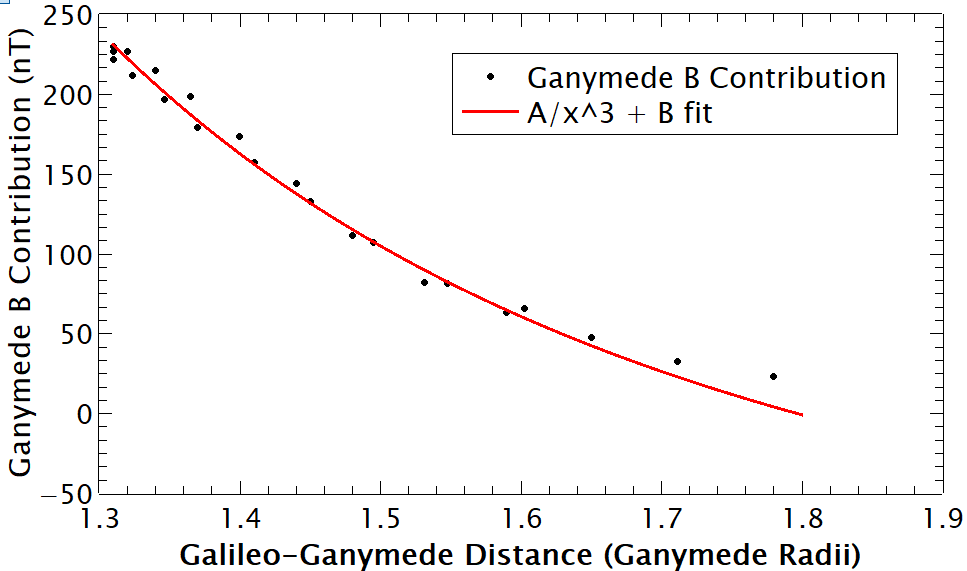
\includegraphics[width=8cm]{MayDist-Mag.png}
    \captionsetup{width=13cm}
    \caption{A plot of Ganymede's isolated magnetic field contribution observed at Galileo (measured in nT) against its distance from the spacecraft (measured in Ganymede radii) for its May 2000 flyby of the moon. A fit has been applied with the equation $\frac{A}{x^{3}} + B$, with determined parameters $A = 850 \pm 20\,nT\,R_{G}^{3}$ and $B = -146 \pm 8\,nT$.}
    \label{fig:MayDist-Mag}
\end{figure}

\noindent The fit parameters in figure \ref{fig:MayDist-Mag} were used to extrapolate and estimate the magnetic field of Ganymede at its surface (i.e. 1 Ganymede radius). The surface magnetic field strength was calculated to be $700 \pm 20$ nT.

Whilst it is evident from figure \ref{fig:flybytrajectory} that the May flyby's closest approach was near to the equatorial plane, Galileo's latitude with respect to Ganymede was not exactly 0\degree, and Ganymede's magnetic field is rotated by 176\degree\,as previously discussed. Therefore, the value from literature of surface magnetic field strength at the equator of 719 nT must be modified to be suitable for Galileo's magnetic colatitude during the May 2000 flyby, using equation \ref{equ:ColatB} to calculate expected magnetic field strength where $B$ is magnetic field strength, $M$ is the dipole magnetic moment ($719\,nT/R_{G}^{3}$ for Ganymede \cite{magrotation}), $r$ is the distance from Ganymede (1 Ganymede radius at the surface) and $\theta$ is the magnetic colatitude \cite{flybylines}.

\begin{equation}
\label{equ:ColatB}
    B = M r^{-3} (1+3\cos{(\theta)}^{2})^{\frac{1}{2}}
\end{equation}

Reading from figure \ref{fig:flybytrajectory}, it can be seen that at closest approach during the May 2000 flyby, Galileo GPhiO coordinates are ($-1.2 \pm 0.2$, $0$, $-0.4 \pm 0.1$) with units of Ganymede radii R$_{G}$, where estimated uncertainties arise due to human error in reading from the plots. These coordinates indicate that during the flyby, Galileo flew to the south of the Geographical equator, and was trailing Ganymede's direction of motion. Equation \ref{equ:ColatXZ} was then used to calculate the geographic colatitude of Galileo with respect to Ganymede to be $\theta_{geo} = -71.57\degree \pm 0.02\degree$.

\begin{equation}
\label{equ:ColatXZ}
    |\theta| = 90\degree - \arctan{\frac{Z}{X}}
\end{equation}

The $176\degree \pm 1$\degree\, rotation of Ganymede's magnetic field with respect to the spin axis would place the magnetic North and South poles of Ganymede at an offset of $\theta_{offset} = 4\degree \pm 1\degree$ from the South and North geographic poles respectively. Therefore, equation \ref{equ:MagColat} can be used to calculate Galileo's magnetic colatitude $\theta_{mag}$ (that is, its colatitude with respect to the magnetic field orientation) by taking the resultant of both angles.

\begin{equation}
\label{equ:MagColat}
    |\theta_{mag}| = \sqrt{|\theta_{geo}|^{2} + |\theta_{offset}|^{2}}
\end{equation}

The magnetic colatitude of Galileo's closest approach to Ganymede, with propagated error, was calculated as $72\degree \pm 18\degree$. The colatitude is positive as whilst the flyby was south of the geographic equator, the 176\degree\, rotation of the magnetic field resulted in Galileo being in the magnetic north. This value was then used in equation \ref{equ:ColatB} to estimate the expected surface magnetic field strength contribution from Ganymede at Galileo's magnetic colatitude as $820 \pm 40$ nT. Using combined error $\sigma$, our obtained result of $700 \pm 20$ nT is therefore 2.67$\sigma$ away from the expected value, suggesting that there is some evidence that the two values are different, but further research should be done to investigate whether such difference is real.

\subsection{Analysis of Ganymede surface magnetic field strength near a pole}

A plot of Ganymede's magnetic field strength against Galileo-Ganymede distance was then produced for the December 2000 flyby data, shown in figure \ref{fig:DecDist-Mag}, showing very similar behaviour to the May 2000 flyby data.

\begin{figure}[!htb]
    \centering
    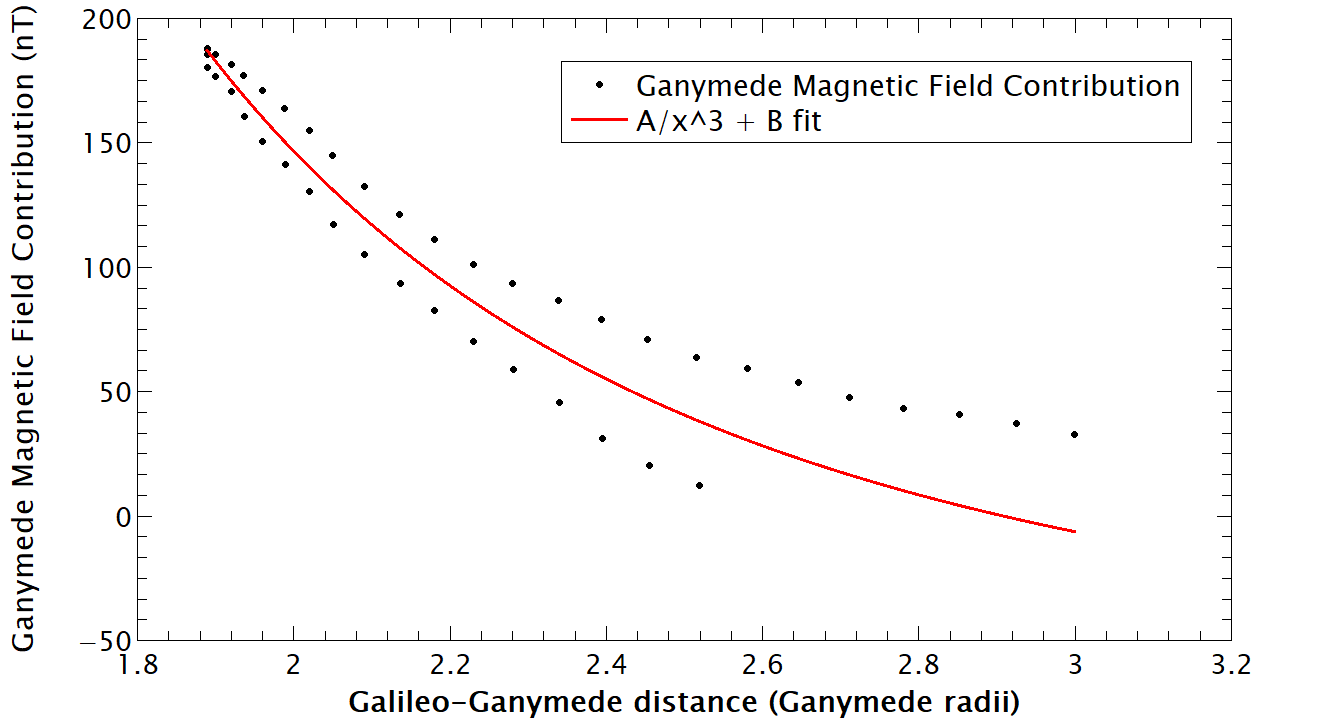
\includegraphics[width=8cm]{DecDist-Mag.png}
    \captionsetup{width=13cm}
    \caption{A plot of Ganymede's isolated magnetic field contribution observed at Galileo (measured in nT) against its distance from the spacecraft (measured in Ganymede radii) for its December 2000 flyby of the moon. A fit has been applied with the equation $\frac{A}{x^{3}} + B$, with determined parameters $A = 1740 \pm 90\,nT\,R_{G}^{3}$ and $B = -71 \pm 11\,nT$.}
    \label{fig:DecDist-Mag}
\end{figure}

\noindent Using the parameters of the applied fit, which appear to represent the data well, it was estimated that the magnetic field of Ganymede at the surface was $1670 \pm 90$ nT. The December 2000 flyby flew over the geographic north pole of the moon, trailing its motion, with closest-approach GPhiO coordinates of ($0.9\pm0.2$, 0, $1.7\pm0.2$) R$_{G}$ \cite{flybylines} so we would expect a greater magnetic field contribution to that at the equator. 

Recorded Galileo-Ganymede latitude data was available for the December flyby which placed the spacecraft's closest approach at a geographic colatitude of $\theta_{geo} = 28\degree \pm 2\degree\,$ \cite{amda}, with error arising due to uncertainty in the human reading from the timeseries. This was then combined with the discussed magnetic field rotation $\theta_{offset}$ in equation \ref{equ:MagColat} to give a magnetic colatitude of $28\degree \pm 7\degree$, corresponding to an expected surface magnetic field strength of $1400 \pm 100$ nT from equation \ref{equ:ColatB}. Therefore, our result of 1670 nT is 2$\sigma$ away from the expected value, where $\sigma$ is combined error, and there is some evidence to suggest a difference in the two values. As with the near-equatorial value obtained from the May 2000 flyby data, further research must be done to conclude which value is correct.

%REFERENCES PAGE
\newpage
\bibliographystyle{unsrt}
\bibliography{bibliography.bib}

\newpage
\appendix
\section{Python Scripts}
\label{app:scripts}
Python script(s) for identifying occasions with a similar Galileo position to December 2000's flyby: \url{https://github.com/IMAGINE-Lancaster-University/IMAGINE/tree/main/Data\%20Python\%20Scripts/JSOpositiondata}.

\noindent Python script(s) for constructing artificial magnetic field data and removing Jupiter's magnetic field contribution: \url{https://github.com/IMAGINE-Lancaster-University/IMAGINE/tree/main/Data\%20Python\%20Scripts/GanymedeIsolation}.

\end{document}
